\documentclass[12pt]{article}
\usepackage[a4paper, total={5.5in, 9in}]{geometry}
\usepackage{amsmath}
\usepackage{amsfonts}
\usepackage{graphicx}
\usepackage{enumitem}
\usepackage{hyperref}

\title{Pre-Statistics Worksheet 6}
\author{PCL Learning Center}
\date{}

\begin{document}
\maketitle

\subsection*{Problem 1}
Solve the equation using the Division and Multiplication Properties of Equality and check the solution:  
\[
-20 = \dfrac{x}{-4}
\]

\subsection*{Problem 2}
Solve the linear equation:  
\[
-2(a - 6) = 4(a - 3)
\]

\subsection*{Problem 3}
Solve the linear equation:  
\[
4(x + 3) = 2(x - 1)
\]

\subsection*{Problem 4}
Solve the following equation with variables and constants on both sides:  
\[
3x - 16 = 2x + 2
\]

\subsection*{Problem 5}
The graph represents the allowable heights \(x\), in inches, of riders on the Whiplash roller coaster.  
Write the inequality represented by the graph.

\begin{figure}[!ht]
    \centering
    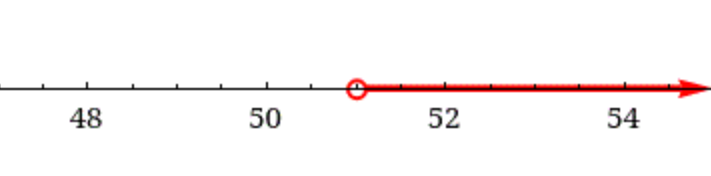
\includegraphics[width=0.5\linewidth]{2.png}
\end{figure}

\subsection*{Problem 6}
Express the inequality \(x > 1\) in interval notation.

\subsection*{Problem 7}
Use interval notation to express the inequality:  
\(x \leq 10\)

\subsection*{Problem 8}
What is the interval notation for the set \(\{x : -10 \leq x < 7\}\)?

\subsection*{Problem 9}
Express the inequality \(5 < x \leq 7\) using interval notation.

\subsection*{Problem 10}
Write the solution set in set-builder notation:  
\[
(-\infty, -3] \cup [-1, \infty)
\]

\subsection*{Problem 11}
Graph \(x > -1\) and \(x \leq 6\) on a number line.

\subsection*{Problem 12}
Write the interval \([2, 11]\) in set-builder notation.

\subsection*{Problem 13}
Solve the linear equation:  
\[
5(x - 2) = 3x + 4
\]

\subsection*{Problem 14}
Write the interval \((-4, 8]\) using set-builder notation.

\subsection*{Problem 15}
Express the inequality \(x \geq -2\) in interval notation and graph it on a number line.

\subsection*{Problem 16}
Solve the equation:  
\[
-3x + 6 = 15
\]

\subsection*{Problem 17}
Write the set-builder notation for the interval \((-\infty, 2] \cup [5, \infty)\).

\subsection*{Problem 18}
Graph the inequality \(x < -4 \text{ or } x > 3\) on a number line.

\subsection*{Problem 19}
Solve the compound inequality and express the solution in interval notation:  
\[
-2 \leq \dfrac{2x - 6}{4} < 3
\]

\subsection*{Problem 20}
Solve the equation and check your solution:  
\[
\dfrac{3x + 1}{2} - \dfrac{x - 4}{3} = \dfrac{5}{6}
\]


\end{document}
